\section{Currently Implemented Solutions}
In his 2018 testimony to congress, Mark Zuckerberg agreed that the current process with content reviewers had room for improvement, saying "... unfortunately, with the amount of content in our systems and the current systems that we have in place to review, we make a relatively small percent of mistakes in content review but that is too many, and this is an area where we need to improve" \citep{energy2018facebook}, and then pivoted to discussing the need for AI solutions. In his 2020 testimony to congress, Zuckerberg stated that they had tripled the security team to 35,000 employees, that they're funding new security technologies to prevent emerging fake threats such as "deep fakes", and that they have implemented resource centers for hot button topics like COVID-19 and the 2020 election \citep{zuckerberg2020}.

\subsection{Current Solution}
As Zuckerberg admitted in 2018, scale is an issue. Facebook currently has a preemptive solution and a two step solution:
\renewcommand{\labelenumii}{\Roman{enumii}}
\begin{enumerate}
\item The preemptive solution is to add a “context” button to all political posts, which a user can click on for more information \citep{smith2018designing}.
 \item If a post has been shared and is untrue, the following steps must be taken before Facebook will flag a post as false:
 \begin{enumerate}
     \item It requires an outside individual to report the post. 
     \item After the post is reported, then it is  sent to 3rd-party fact checkers for verification. 
     \item Third party fact checkers must log in to the Facebook dashboard and then provide a link proving the story is false (they cannot simply mark a story as untrue).
 \end{enumerate}
 \end{enumerate}
 
 In Facebook’s case, after they have determined a particular post is false, then the post is shown less frequently (80 percent less), other posts of the same link or image will also be shown less, it will be unable to be converted into an ad later, and someone re-sharing this post will be given a notification that the information is likely false \citep{owen2016clamping,facebook_2020}.
 
 The punishment for routine offenders or for routine fake stories that point to a common domain is a loss of advertising rights and a loss of ability to monetize \citep{facebook_2020}.
 
 \subsection{Issues with Preemptive Solution}
 The "context" button is ineffective for several reasons. 
 
 First, it assumes that people will actively search for context when viewing a link. People are unlikely to feel the need to do further research if they agree with or believe the headline as presented \citep{nyhan2010corrections}. This problem is augmented by the fact that headlines are often misleading and written to draw the strongest possible emotional response \citep{chesney2017incongruent,ecker2014effects,bell1984good,molek2013towards,kilgo2018new,vettehen2008explaining}. For example with the \textit{Express} newspaper from the UK (from Ecker, et al.):
 \begin{itemize}
 \item Headline: Air pollution now leading cause of lung cancer
\item Evidence within article: “We now know that outdoor air pollution is not only a major risk to health in general, but also a leading \textbf{environmental} cause of cancer deaths.” Dr. Kurt Straif, of IARC [emphasis added]
 \end{itemize}
 
 Or from the \textit{Independent}'s Facebook page \citep{chesney2017incongruent}:
 \begin{itemize}
\item Social media post copy: Enjoy it while you
can
\item Social media headline\footnote{https://www.facebook.com/TheIndependentOn-line/posts/10154972799736636}: Scientists have predicted the end of sex
\item Article headline\footnote{Will Worley (2016): http://www.independent.co.uk/news/science/sex-unnecessary-designer-babies-stanfordprofessor-says-a6957636.html}: Sex will be made unnecessary by ‘designer babies’, professor says
\item Evidence within article: Professor Henry Greely believes that in as little as 20 years, most children will be conceived in a laboratory, rather than through sexual intercourse.
 \end{itemize}
 
 While there have been attempts to track down misleading headlines, they have primarily centered around \textit{click-bait} or tabloid headlines \citep{chen2015misleading,chakraborty2016stop}that require the user to click to find out the information, e.g. "Here’s What Happens When You Put A Few Little Kids In A Room With 2 Dolls In 2 Different Colors" \citep{chen2015misleading}. While this will help with some problems, both the \textit{Express} and \textit{The Independent} articles would not be caught by the proposed algorithms. 
 
 Furthermore, In fact, only 59 percent of all shared URLs are ever clicked on Twitter \citep{gabielkov2016social}, which has led to Twitter adding in features that prompt users to read articles rather than just headlines before sharing the article \citep{reuters2020article}. Unsurprisingly, the backlash was immediate:
 \begin{figure}[htp]
    \centering
    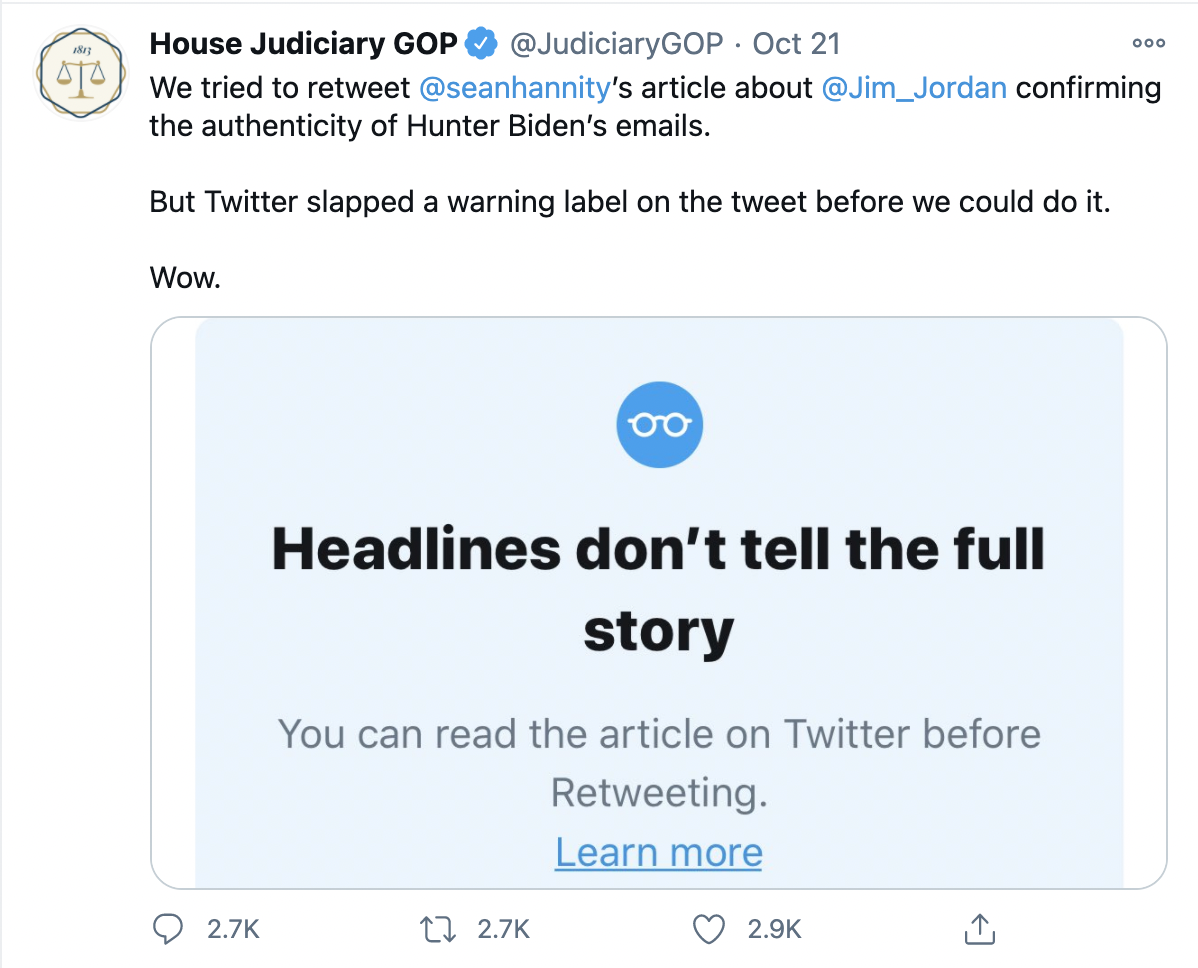
\includegraphics[width=4cm]{JudiciaryTweet.png}
    \caption{House Judiciary GOP Tweet}
    \label{fig:House Judiciary GOP Tweet}
\end{figure}
As will be discussed shortly, this fits the problem of \textit{echo chambers} wherein the primary question is not "is this correct" but "does it align with the views of me and my group?" 

To summarize, the proposed preemptive solution is ineffective because:
\being{itemize}
\item 41 percent of the time, someone will retweet an article without having read more than the headline. \citep{gabielkov2016social}
\item Headlines are written to be intentionally misleading, or at least to generate a strong emotional response from the reader.\citep{chesney2017incongruent}
\item Readers are unlikely to fact-check, question, or feel compelled to do outside research on an article if the have a strong emotional response to it.\citep{nyhan2010corrections}
 
 \subsection{Issues with Two Step Solution}
 The key first step for this solution is that an individual must report the post as false. This requires a level of self policing that it is unlikely given the prevalence of \textit{echo chambers}. 
 
 Because social media seeks to connect like minded individuals, it has a tendency to generate \textit{echo chambers}, or closed networks with high repetition of content and low diversity of thought \citep{adibi2005proceedings, bastian2009international, pariser2011filter,bozdag2015breaking}. While not every closed homogeneous network is inherently bad -- they can operate as self-help groups \citep{kast2012under} or can encourage positive behavior like reducing prejudice \citep{paluck2011peer} -- there is a clear and well documented history that people are influenced by others in their network \citep{bollinger2012peer, bond201261,gerber2008social,gerber2009descriptive,meer2011brother,paluck2012salience,del2016spreading,bessi2015viral} and this can be destructive in the context of misinformation. For this paper's purposes, $a_k$, the partisan leaning of some user $u_k$ is directly proportional to the partisan leaning of the network $N_k$ and can be described as follows:
 \begin{equation}
    \label{leaningproportionaltonetwork}
     a_k \propto \frac{\Sigma_{n=1}^{|N_k|}{a_n}}{|N_k|}
 \end{equation}
 
 For validation of this, in Bullock's experiments he found that participants would change their opinions on a particular topic if they were told that the party they identify with held an opposing view, even if it was counter-intuitive, such as a Republican being told that the Republican party was against a conservative initiative \citep{bullock2007experiments}. Other research provides similar results: Republicans and Democrats are likely to accept a statement as being true and not feel the need to research personally if it comes from a preferred politician \cite{housholder2014facebook}; even if a preferred politician's statements are disproved, there is no shift in voting intentions, party identification, or overall perceived credibility of that politician \citep{swire2017processing}. 
 
 Further complicating the situation, closed networks are likely to be more resistant to fact-checking or corrective information coming from outside of their network \citep{garrett2013undermining,lord1979biased,edwards1996disconfirmation,redlawsk2002hot, taber2006motivated}. This explains why even the release of President Obama's long form birth certificate only briefly quieted the conspiracy that he was not born in the United States \citep{nyhan2012new} -- so long as the corrective information came from outside of the echo-chamber, it was fundamentally dismissed.
 
 Unsurprisingly, these closed groups are more than eager to fact-check individuals who do not belong to their group, such as Republicans fact checking Democrats and vice-versa \citep{shin2017partisan,iyengar2015fear}.

\subsection{partisanship} 
There is substantial research that Americans who identify as right-wing have historically been more susceptible than other subsets of the American population to fake news \citep{guess2019less,benkler2018network,grinberg2019fake,allcott2017social,badawy2018analyzing}, more thorough analysis suggests that this pattern may not hold up moving forward.

First, a better predictor of willingness to share misinformation is general distrust in the media rather than political leaning \citep{hopp2020people,shin2017partisan,kahan2012ideology,lewandowsky2016motivated,swire2017processing,mourao2019fake}. This is further born out by the Russian "troll farm" known as the Internet Research Agency (IRA) heavily targeting three groups they determined were unlikely to trust the main stream media: far right-wing Americans, far left-wing Americans, and Black Americans \citep{diresta2019tactics,howard2019ira,boatwright2018troll,jamieson2020cyberwar}. 

Second, many of these individuals are more focused on empathy with a particular group \citep{rheault2016measuring,dale2017nlp} or engaging in signaling theory with a group \citep{connelly2011signaling,lampe2007familiar,spence2002signaling} rather than objective truth. Dominic Cummings callously stated while creating inaccurate content for the Leave campaign for Brexit that "accuracy is for snake-oil pussies" \citep{crace2016accuracy}, yet his point is widespread and in line with the analysis of \textit{echo chambers}: in hyper-partisan situations, strongly held opinions that are counter to widely accepted narratives are seen primarily as signals of commonality \citep{yla2018populist,noppari2019user,lazer2018science,yla2019politicization,wasilewski2019us}. 

Third, there is no difference in propensity to share non-partisan misinformation, such as the dangers of living near power lines or the side-effects of MMR vaccines, between people of various beliefs \citep{kahan2015climate,hara2016co}.

Finally, most of the studies referenced previously looked at data from 2016 and before. Since 2016, there has been a well documented global rise in populism on both ends of the political spectrum, such that members on these fringes have disproportionately large blocs on social media in comparison to their actual presence as seen in the French 2017 election \citep{donadio2017french,vinocur2017marine} and the 2015 EU Parliament:  \begin{figure}[htp]
    \centering
    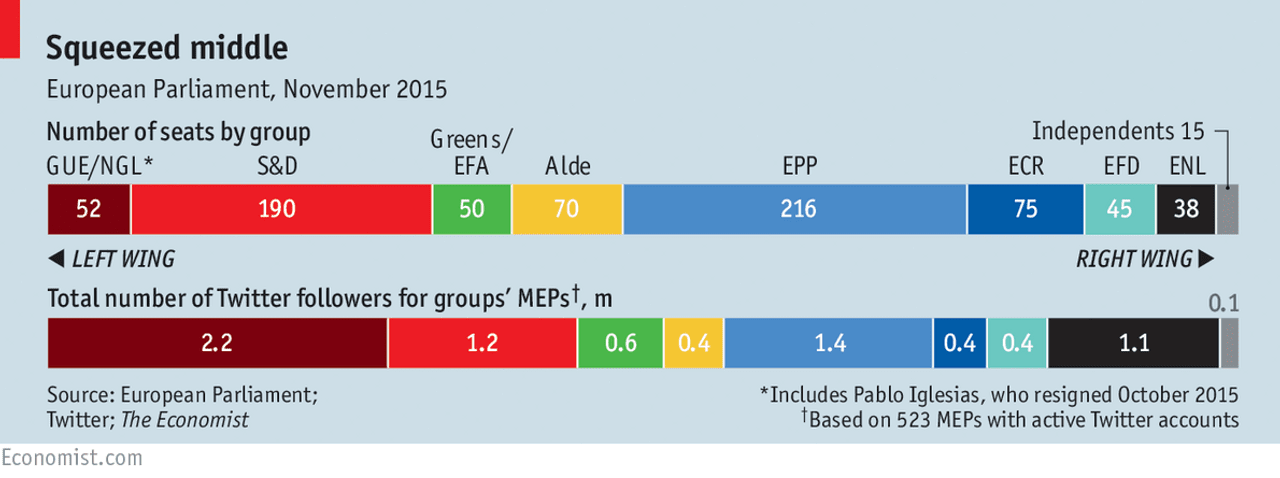
\includegraphics[width=4cm]{European Parliament 2015.png}
    \caption{Breakdown of European Parliament 2015 from The Economist, seats vs. millions of followers}
    \label{img:European Parliament 2015}
\end{figure}
 
 \subsection{Third Party Fact Checkers}
 The usage of third party fact checkers has two fundamental issues.
 
 First, there is a large volume of research over decades that ideologues on either side of the political spectrum will view the exact same content as being biased against them \citep{arpan2003experimental,baum2008eye,christen2002hostile,gunther2001predicting,gunther2004mapping,baum2004issue,gussin2004eye,lee2005liberal,vallone1985hostile}. This is extending to fact-checking, as groups on both the left and the right post about claims of censorship when their content is removed or their reach is reduced \citep{Dreyfuss2020Now,Post2020Facebook,Millhiser2018Facebook}. 
 
 As Shin and Thorson noted, however, closed networks are eager to fact check members who are not of their group. In 2018, Think Progress (a liberal Facebook fact checker) had an article on the Brett Kavanaugh Supreme Court confirmation hearing that was flagged as false by The Weekly Standard (a conservative Facebook fact checker) \citep{owen2018with}. Think Progress stated that then-Judge Kavanaugh had said during his hearing that he would kill Roe v. Wade \citep{millhiser2018brett}, a claim that was deemed false by the Weekly Standard and by FactCheck.org, a non-partisan fact-checking organization \citep{gore2018kavanaugh}. The Weekly Standard offered to remove its flag if Think Progress replaced the word "said" in the headline, as Judge Kavanaugh had not explicitly said that he would overturn Roe v. Wade. Think Progress argued that secondary and tertiary definitions of "said" made their headline correct, and instead accused Facebook of bias \citep{legum2018tweet}. Shortly after, several other liberal journalists made the same argument, with none touching on whether or not the word "said" was truthful \citep{froomkin2018tweet,grim2018tweet,beutler2018tweet}. 
 
It is unsurprising that fact checkers are susceptible to the same \textit{echo chamber} behavior discussed previously, and it echoes the problem posed by Juvenal in his Satires: "Who will watch the watchmen?" 

Second, high quality non-partisan fact checkers, such as Snopes and the Associated Press have left their fact checking partnership with Facebook or stopped working as Facebook's process is manual, time consuming, ineffective, and does not provide adequate compensation for the time required to do the job thoroughly \citep{green2019message,coldeway2019update}. Since there is no appeals process for an article being flagged and removed by a third party fact checker, it would be incredibly easy for an ideologue to censor opposing viewpoints: after the Think Progress/Weekly Standard argument, there would be nothing stopping Think Progress from flagging every single article that the Weekly Standard ever posted in the future as retaliation. As shown in game theory applications with censorship, the probabilities of winning decrease from 37 percent to 28 percent to 22 percent as censorship becomes more restrictive \citep{dotsenko2013censorship}.